\documentclass[12pt,a4paper,oneside]{report}

% ------------------------------------------------------------------------------
% CẤU HÌNH ĐỊNH DẠNG THEO QUY ĐỊNH KHOA CNTT - ĐẠI HỌC XÂY DỰNG HÀ NỘI
% ------------------------------------------------------------------------------
\usepackage{iftex}
\ifPDFTeX
  \usepackage[utf8]{inputenc}
  \usepackage[vietnamese]{babel}
  \usepackage{mathptmx} % Times New Roman
\else
  \usepackage{fontspec}
  \setmainfont{Times New Roman}
\fi

\usepackage[a4paper,
  left=3.5cm,
  right=2.0cm,
  top=2.5cm,
  bottom=2.5cm
]{geometry}

\usepackage{graphicx}
\usepackage{amsmath,amssymb}
\usepackage{booktabs}
\usepackage{tabularx}
\usepackage{array}
\usepackage{caption}
\usepackage{subcaption}
\usepackage{fancyhdr}
\usepackage{titlesec}
\usepackage{setspace}
\usepackage{hyperref}
\usepackage{listings}
\usepackage{xcolor}

% Thiết lập dãn dòng 1.2 theo quy định
\setstretch{1.2}

% Định nghĩa màu sắc
\definecolor{HuceBlue}{RGB}{0, 43, 91}
\definecolor{codegreen}{rgb}{0,0.6,0}
\definecolor{codegray}{rgb}{0.5,0.5,0.5}
\definecolor{codepurple}{rgb}{0.58,0,0.82}
\definecolor{backcolour}{rgb}{0.96,0.96,0.96}

% Cấu hình code listing
\lstdefinestyle{mystyle}{
    backgroundcolor=\color{backcolour},   
    commentstyle=\color{codegreen},
    keywordstyle=\color{HuceBlue}\bfseries,
    numberstyle=\tiny\color{codegray},
    stringstyle=\color{codepurple},
    basicstyle=\ttfamily\footnotesize,
    breakatwhitespace=false,         
    breaklines=true,                 
    captionpos=b,                    
    keepspaces=true,                 
    numbers=left,                    
    numbersep=5pt,                  
    showspaces=false,                
    showstringspaces=false,
    showtabs=false,                  
    tabsize=2
}
\lstset{style=mystyle}

% Cấu hình header & footer
\pagestyle{fancy}
\fancyhf{}
\fancyhead[R]{\textit{\small Ứng dụng Học máy trong phát hiện Botnet từ lưu lượng mạng}}
\fancyfoot[R]{\thepage}
\renewcommand{\headrulewidth}{0.4pt}
\renewcommand{\footrulewidth}{0pt}

% Cấu hình định dạng tiêu đề chương, mục (Tối đa 3 cấp theo quy định)
\titleformat{\chapter}[hang]{\normalfont\LARGE\bfseries\color{HuceBlue}}{\thechapter.}{0.5em}{}
\titlespacing*{\chapter}{0pt}{-10pt}{20pt}
\titleformat{\section}{\normalfont\Large\bfseries\color{HuceBlue}}{\thesection}{0.5em}{}
\titleformat{\subsection}{\normalfont\large\bfseries}{\thesubsection}{0.5em}{}
\titleformat{\subsubsection}{\normalfont\normalsize\bfseries}{\thesubsubsection}{0.5em}{}

% Đường dẫn hình ảnh
\graphicspath{{./}{output_charts/}}

\begin{document}

% ==============================================================================
% [SECTION 1] TRANG BÌA VÀ LỜI MỞ ĐẦU
% ==============================================================================
\begin{titlepage}
  \thispagestyle{empty}
  \begin{center}
    {\large \textbf{TRƯỜNG ĐẠI HỌC XÂY DỰNG HÀ NỘI}}\\[0.2cm]
    {\large \textbf{KHOA CÔNG NGHỆ THÔNG TIN}}\\[0.1cm]
    {\normalsize \textbf{BỘ MÔN KỸ THUẬT HỆ THỐNG}}\\[0.2cm]
    \textbf{-------------o0o-------------}\\[1.2cm]

    \IfFileExists{logo_huce.png}{
      
\includegraphics[height=3.2cm]{logo_huce.png}\\[1.2cm]
    }{
      \vspace{3.5cm}
    }

    {\Large \textbf{BÁO CÁO BÀI TẬP LỚN}}\\[0.2cm]
    {\normalsize \textbf{HỌC PHẦN: AN TOÀN VÀ BẢO MẬT THÔNG TIN}}\\[0.5cm]

    \vspace{0.5cm}
    {\LARGE \textbf{\color{HuceBlue} ỨNG DỤNG HỌC MÁY TRONG PHÁT HIỆN BOTNET TỪ LƯU LƯỢNG MẠNG}}\\[1.5cm]

    \begin{minipage}{0.9\textwidth}
      \begin{tabular}{lll}
        \textbf{Giảng viên hướng dẫn:} & \multicolumn{2}{l}{\textbf{ThS. Nguyễn Việt Nhật}} \\[0.3cm]
        \textbf{Sinh viên thực hiện:}  & Nguyễn Bá Hùng & \textbf{MSV: 0368269} \\
                                       & Nguyễn Duy Hùng & \textbf{MSV: 0368369} \\
                                       & Lê Quang Huy   & \textbf{MSV: 0368469} \\
                                       & Ngô Xuân Trung & \textbf{MSV: 0373569} \\
                                       & Bùi Đức Thắng  & \textbf{MSV: 0373069} \\[0.2cm]
        \textbf{Ngành:}                & \multicolumn{2}{l}{Công nghệ Thông tin} \\
      \end{tabular}
    \end{minipage}

    \vfill
    {\large \textbf{HÀ NỘI -- 2026}}
  \end{center}
\end{titlepage}

% TRANG BÌA PHỤ
\newpage
\thispagestyle{empty}
\begin{center}
  {\large \textbf{TRƯỜNG ĐẠI HỌC XÂY DỰNG HÀ NỘI}}\\[0.2cm]
  {\large \textbf{KHOA CÔNG NGHỆ THÔNG TIN}}\\[0.2cm]
  \textbf{-------------o0o-------------}\\[1.0cm]

  \IfFileExists{logo_huce.png}{
    
\includegraphics[height=2.5cm]{logo_huce.png}\\[1.0cm]
  }{
    \vspace{2.5cm}
  }

  {\Large \textbf{BÁO CÁO BÀI TẬP LỚN}}\\[0.3cm]
  {\normalsize \textbf{NGÀNH: CÔNG NGHỆ THÔNG TIN}}\\[0.8cm]

  {\Large \textbf{\color{HuceBlue} ỨNG DỤNG HỌC MÁY TRONG PHÁT HIỆN BOTNET TỪ LƯU LƯỢNG MẠNG}}\\[1.5cm]

  \begin{minipage}{0.9\textwidth}
    \begin{tabular}{lll}
      \textbf{Giảng viên hướng dẫn:} & \multicolumn{2}{l}{\textbf{ThS. Nguyễn Việt Nhật}} \\[0.3cm]
      \textbf{Sinh viên thực hiện:}  & Nguyễn Bá Hùng & \textbf{MSV: 0368269} \\
                                     & Nguyễn Duy Hùng & \textbf{MSV: 0368369} \\
                                     & Lê Quang Huy   & \textbf{MSV: 0368469} \\
                                     & Ngô Xuân Trung & \textbf{MSV: 0373569} \\
                                     & Bùi Đức Thắng  & \textbf{MSV: 0373069} \\
    \end{tabular}
  \end{minipage}

  \vfill
  {\large \textbf{HÀ NỘI -- 2026}}
\end{center}

% LỜI CAM ĐOAN
\newpage
\chapter*{LỜI CAM ĐOAN}
\addcontentsline{toc}{chapter}{Lời cam đoan}
Nhóm chúng em xin cam đoan bản báo cáo bài tập lớn đề tài \textit{"Ứng dụng Học máy trong phát hiện Botnet từ lưu lượng mạng"} là công trình nghiên cứu do tập thể nhóm sinh viên chúng em cùng tìm hiểu, nghiên cứu và thực hiện dưới sự định hướng, hướng dẫn khoa học của Thầy \textbf{ThS. Nguyễn Việt Nhật}.

Các số liệu thực nghiệm, kết quả mô phỏng và biểu đồ được tạo ra trực tiếp từ mã nguồn thực thi trên tập dữ liệu chuẩn quốc tế CTU-13. Toàn bộ các thông tin, tài liệu tham khảo được trích dẫn trong báo cáo đều có nguồn gốc rõ ràng theo đúng chuẩn học thuật của Nhà trường và Khoa Công nghệ Thông tin. Nhóm tác giả xin hoàn toàn chịu trách nhiệm trước Nhà trường nếu có bất kỳ sự gian lận hoặc sao chép trái phép nào.

\vspace{1.5cm}
\begin{flushright}
  \textit{Hà Nội, ngày 17 tháng 09 năm 2026}\\[0.3cm]
  \textbf{Đại diện nhóm sinh viên thực hiện}\\[1.5cm]
  \textbf{Nguyễn Bá Hùng}
\end{flushright}

% LỜI CẢM ƠN
\newpage
\chapter*{LỜI CẢM ƠN}
\addcontentsline{toc}{chapter}{Lời cảm ơn}
Lời đầu tiên, nhóm chúng em xin gửi lời cảm ơn sâu sắc nhất tới các Thầy/Cô giáo trong Khoa Công nghệ Thông tin - Trường Đại học Xây dựng Hà Nội, những người đã trang bị cho chúng em nền tảng kiến thức vững chắc về mạng máy tính, an toàn thông tin và trí tuệ nhân tạo trong suốt quá trình học tập.

Đặc biệt, nhóm chúng em xin bày tỏ lòng biết ơn chân thành và sâu sắc nhất tới Thầy \textbf{ThS. Nguyễn Việt Nhật} – Giảng viên trực tiếp giảng dạy và hướng dẫn học phần An toàn và Bảo mật thông tin. Thầy đã luôn định hướng đề tài thực tế, tận tình chỉ dẫn và đóng góp những ý kiến học thuật quý báu giúp nhóm hoàn thiện quy trình nghiên cứu, xây dựng mô hình và đánh giá hiệu năng hệ thống một cách khoa học.

Dù các thành viên trong nhóm đã nỗ lực hết sức để hoàn thành báo cáo một cách chỉn chu nhất, song do thời gian và kiến thức còn hạn chế nên báo cáo khó tránh khỏi những thiếu sót. Nhóm chúng em rất mong nhận được những nhận xét, góp ý quý báu từ Thầy để đề tài ngày càng hoàn thiện hơn.

\vspace{1.5cm}
\begin{flushright}
  \textbf{Tập thể nhóm sinh viên thực hiện}\\[0.5cm]
  \textit{Nguyễn Bá Hùng -- Nguyễn Duy Hùng -- Lê Quang Huy}\\
  \textit{Ngô Xuân Trung -- Bùi Đức Thắng}
\end{flushright}

% ==============================================================================
% [SECTION 2] MỤC LỤC & DANH MỤC
% ==============================================================================
\newpage
\pagenumbering{roman}
\tableofcontents

\newpage
\chapter*{DANH MỤC TỪ VIẾT TẮT, THUẬT NGỮ}
\addcontentsline{toc}{chapter}{Danh mục từ viết tắt, thuật ngữ}
\begin{table}[h]
\centering
\begin{tabular}{|c|l|p{8.5cm}|}
\hline
\textbf{STT} & \textbf{Từ viết tắt} & \textbf{Giải nghĩa tiếng Việt / Tiếng Anh} \\ \hline
1 & AI & Artificial Intelligence (Trí tuệ nhân tạo) \\ \hline
2 & ATTT & An toàn thông tin \\ \hline
3 & Bwd & Backward (Chiều gói tin phản hồi từ đích về nguồn) \\ \hline
4 & C2 & Command and Control (Kênh chỉ huy và điều khiển mã độc) \\ \hline
5 & CIC & Canadian Institute for Cybersecurity (Viện An ninh mạng Canada) \\ \hline
6 & CTU & Czech Technical University (Đại học Kỹ thuật Séc) \\ \hline
7 & DDoS & Distributed Denial of Service (Tấn công từ chối dịch vụ phân tán) \\ \hline
8 & DPI & Deep Packet Inspection (Kỹ thuật soi sâu nội dung gói tin) \\ \hline
9 & Flow & Luồng mạng hai chiều giữa hai thực thể truyền thông \\ \hline
10 & Fwd & Forward (Chiều gói tin truyền từ nguồn đến đích) \\ \hline
11 & IAT & Inter-Arrival Time (Thời gian cách quãng giữa hai gói tin) \\ \hline
12 & IDS & Intrusion Detection System (Hệ thống phát hiện xâm nhập) \\ \hline
13 & IPS & Intrusion Prevention System (Hệ thống ngăn ngừa xâm nhập) \\ \hline
14 & ML & Machine Learning (Học máy) \\ \hline
15 & PCAP & Packet Capture (Tập tin định dạng bắt gói tin mạng thô) \\ \hline
16 & RF & Random Forest (Thuật toán Rừng ngẫu nhiên) \\ \hline
17 & ROC-AUC & Receiver Operating Characteristic - Area Under Curve \\ \hline
18 & SYN & Synchronize (Cờ bắt tay khởi tạo kết nối trong giao thức TCP) \\ \hline
19 & TLS & Transport Layer Security (Giao thức bảo mật tầng truyền vận) \\ \hline
20 & Zero-day & Lỗ hổng hoặc biến thể mã độc mới chưa có chữ ký nhận diện \\ \hline
\end{tabular}
\end{table}

\newpage
\listoftables
\addcontentsline{toc}{chapter}{Danh mục bảng biểu}

\newpage
\listoffigures
\addcontentsline{toc}{chapter}{Danh mục hình vẽ, đồ thị}

% ==============================================================================
% [SECTION 3] NỘI DUNG CHÍNH CỦA BÁO CÁO
% ==============================================================================
\newpage
\pagenumbering{arabic}

\chapter*{MỞ ĐẦU}
\addcontentsline{toc}{chapter}{Mở đầu}

\textbf{1. Lý do chọn đề tài}

Trong thời đại bùng nổ của chuyển đổi số và Internet kết nối vạn vật (IoT), mạng máy tính ma (\textit{Botnet}) đã trở thành một trong những mối đe dọa nghiêm trọng nhất đối với an ninh không gian mạng toàn cầu. Botnet là công cụ đắc lực được tin tặc sử dụng để thực hiện các chiến dịch tấn công từ chối dịch vụ phân tán (DDoS) quy mô terabit, phát tán thư rác, tống tiền bằng Ransomware và đánh cắp dữ liệu nhạy cảm.

Các hệ thống phát hiện xâm nhập truyền thống (NIDS) dựa trên tập luật (Rule-based) hoặc chữ ký tĩnh (Signature-based) như Snort, Suricata đang đối mặt với những thách thức chí mạng: chúng hoàn toàn bị qua mặt trước các biến thể mã độc mới (\textit{Zero-day}) và bị vô hiệu hóa khi hơn $90\%$ lưu lượng Internet hiện nay đã được mã hóa bằng các giao thức TLS/HTTPS. Do đó, việc chuyển hướng nghiên cứu sang tiếp cận phân tích đặc trưng hành vi luồng mạng (\textit{Flow-based}) kết hợp với các thuật toán Học máy (\textit{Machine Learning}) là xu thế tất yếu, mở ra giải pháp phát hiện botnet hiệu quả, chuẩn xác mà không cần giải mã gói tin.

\textbf{2. Mục tiêu nghiên cứu}
\begin{itemize}
  \item Nghiên cứu cơ chế hoạt động, kiến trúc chỉ huy và điều khiển (C2) của Botnet từ góc độ lưu lượng mạng.
  \item Xây dựng pipeline hoàn chỉnh từ khâu tiếp nhận luồng mạng, trích xuất đặc trưng thống kê hai chiều đến huấn luyện và đánh giá mô hình phân loại.
  \item Thực nghiệm, so sánh hiệu năng của các thuật toán Học máy tiêu biểu (Logistic Regression, Decision Tree, Random Forest) trên bộ dữ liệu chuẩn quốc tế CTU-13.
  \item Phân tích các đặc trưng mạng có tính đóng góp cao nhất và đề xuất giải pháp tối ưu hóa đặc trưng (\textit{Feature Selection}) phục vụ triển khai thời gian thực trên thiết bị mạng.
\end{itemize}

\textbf{3. Bố cục của đồ án}
\begin{itemize}
  \item \textbf{Chương 1:} Tổng quan về Botnet và phương pháp phát hiện từ lưu lượng mạng.
  \item \textbf{Chương 2:} Cơ sở dữ liệu thực nghiệm và các thuật toán Học máy.
  \item \textbf{Chương 3:} Kết quả thực nghiệm, đánh giá và tối ưu hóa hệ thống.
  \item \textbf{Kết luận và Hướng phát triển.}
\end{itemize}

% ------------------------------------------------------------------------------
% CHƯƠNG 1
% ------------------------------------------------------------------------------
\chapter{TỔNG QUAN VỀ BOTNET VÀ PHƯƠNG PHÁP PHÁT HIỆN TỪ LƯU LƯỢNG MẠNG}

\section{Tổng quan về mạng Botnet}
\subsection{Khái niệm và kiến trúc mạng Botnet}
Botnet là một mạng lưới các thiết bị máy tính, máy chủ hoặc thiết bị IoT bị lây nhiễm phần mềm độc hại (Malware) và bị kiểm soát từ xa bởi kẻ tấn công (thường được gọi là \textit{Botmaster}). Mỗi thiết bị bị nhiễm trong mạng lưới được gọi là một \textit{Bot} hay \textit{Zombie}.

Điểm khác biệt căn bản giữa Botnet và các loại phần mềm độc hại độc lập (như virus hay worm truyền thống) là sự tồn tại của hạ tầng \textbf{Chỉ huy và Điều khiển (Command and Control - C2)}. Thông qua kênh C2, Botmaster có thể phát lệnh đồng loạt tới hàng chục nghìn máy nạn nhân để thực hiện các cuộc tấn công phối hợp.

\subsection{Vòng đời hoạt động của Botnet}
Vòng đời của một mạng Botnet tiêu chuẩn trải qua 4 giai đoạn chính:
\begin{enumerate}
  \item \textbf{Lây nhiễm (Infection):} Botmaster quét mạng tìm kiếm các lỗ hổng bảo mật chưa được vá hoặc gửi email lừa đảo (Phishing) để đưa mã độc vào thiết bị đích.
  \item \textbf{Khởi động và Kết nối C2 (Rendezvous):} Sau khi thâm nhập thành công, Bot kích hoạt và thiết lập kết nối bí mật trở lại máy chủ C2.
  \item \textbf{Duy trì và Lắng nghe lệnh (Beaconing/Keep-alive):} Bot định kỳ gửi các gói tin thăm dò tín hiệu (Heartbeat) với kích thước rất nhỏ về máy chủ C2 để báo cáo trạng thái trực tuyến và chờ lệnh.
  \item \textbf{Thực thi tấn công (Execution):} Khi nhận được lệnh từ Botmaster, các bot đồng loạt phát động tấn công (như gửi hàng triệu yêu cầu HTTP Flood làm sập mục tiêu).
\end{enumerate}

\section{Thách thức của các hệ thống IDS truyền thống}
\subsection{Phát hiện dựa trên chữ ký (Signature-based) và DPI}
Các hệ thống phát hiện xâm nhập thế hệ trước chủ yếu dựa vào kỹ thuật soi sâu nội dung gói tin (\textit{Deep Packet Inspection - DPI}). Cơ chế này so khớp các chuỗi nhị phân trong phần dữ liệu tải (Payload) của gói tin với cơ sở dữ liệu chữ ký của các loại mã độc đã biết.

\subsection{Sự sụp đổ của phương pháp DPI trước lưu lượng mã hóa}
Trong môi trường mạng hiện đại, kỹ thuật DPI bộc lộ hai lỗ hổng không thể khắc phục:
\begin{itemize}
  \item \textbf{Mã hóa toàn diện (TLS/HTTPS):} Nội dung gói tin đã bị mã hóa thành chuỗi ngẫu nhiên không thể đọc được. Nếu muốn soi DPI, quản trị viên bắt buộc phải sử dụng các giải pháp giải mã trung gian (SSL Interception/Inspection) – điều này gây vi phạm nghiêm trọng quyền riêng tư của người dùng và làm tăng độ trễ mạng lên gấp nhiều lần.
  \item \textbf{Tấn công Zero-day và Biến thể mới:} Tin tặc liên tục thay đổi mã nguồn (Polymorphic Malware), khiến cơ sở dữ liệu chữ ký luôn đi sau kẻ tấn công.
\end{itemize}

\section{Phương pháp tiếp cận dựa trên Luồng mạng (Flow-based Analysis)}
\subsection{Khái niệm Luồng mạng hai chiều (Bidirectional Flow)}
Một luồng mạng (\textit{Flow}) được định nghĩa là tập hợp các gói tin di chuyển giữa hai điểm cuối truyền thông trong một khoảng thời gian nhất định, được định danh bởi bộ 5 thông số (\textit{5-tuple}):
\begin{equation}
  \text{Flow} = \{ \text{IP}_{\text{src}}, \text{IP}_{\text{dst}}, \text{Port}_{\text{src}}, \text{Port}_{\text{dst}}, \text{Protocol} \}
\end{equation}

\subsection{Lợi thế của đặc trưng thống kê luồng mạng}
Thay vì nhìn vào nội dung gói tin, phương pháp tiếp cận theo luồng trích xuất các đặc trưng siêu dữ liệu thống kê (\textit{Statistical Metadata}):
\begin{itemize}
  \item \textbf{Đặc trưng thời gian:} Tổng thời lượng luồng (\textit{Flow Duration}), khoảng cách thời gian giữa các gói tin liên tiếp (\textit{Inter-Arrival Time - IAT}).
  \item \textbf{Đặc trưng kích thước:} Tổng số byte gửi/nhận, kích thước trung bình và độ lệch chuẩn của gói tin.
  \item \textbf{Đặc trưng trạng thái giao thức:} Số lượng cờ bắt tay (SYN), cờ xác nhận (ACK), cờ ngắt kết nối (RST/FIN).
\end{itemize}
\textit{Ý nghĩa cốt lõi:} Dù mã độc có mã hóa toàn bộ dữ liệu truyền tải, hành vi máy móc (chu kỳ gửi tin định kỳ, tỷ lệ gói tin bất đối xứng, tần suất quét cổng) vẫn in hằn rõ nét trên các thông số thống kê của luồng.

\section{Kết chương}
Chương 1 đã phân tích rõ nguy cơ của Botnet và chỉ ra giới hạn của các phương pháp phát hiện dựa trên chữ ký trước làn sóng mã hóa lưu lượng. Đây là cơ sở khoa học vững chắc để đề tài lựa chọn hướng tiếp cận phân tích đặc trưng luồng mạng kết hợp Học máy làm phương pháp nghiên cứu trọng tâm.

% ------------------------------------------------------------------------------
% CHƯƠNG 2
% ------------------------------------------------------------------------------
\chapter{BỘ DỮ LIỆU THỰC NGHIỆM VÀ CÁC THUẬT TOÁN HỌC MÁY}

\section{Bộ dữ liệu chuẩn quốc tế CTU-13}
\subsection{Bối cảnh thu thập bộ dữ liệu}
Bộ dữ liệu \textbf{CTU-13} được thu thập vào năm 2011 tại Đại học Kỹ thuật Séc (CTU Prague) bởi phòng thí nghiệm \textit{Stratosphere Laboratory} – nhóm nghiên cứu sáng lập hệ thống phòng thủ mã nguồn mở \textit{Stratosphere Linux IPS (Slips)}.

Mục tiêu của bộ dữ liệu là tạo ra một môi trường lưu lượng mạng hỗn hợp thực tế cao, kết hợp giữa lưu lượng người dùng bình thường của trường đại học và lưu lượng của 13 kịch bản mã độc Botnet khác nhau đang hoạt động (như Neris, Rbot, Virut, Donbot, Sogou).

\subsection{Quy trình trích xuất đặc trưng bằng CICFlowMeter}
Các tập tin bắt gói tin mạng thô (\texttt{.pcap}) của CTU-13 được chuyển đổi thành dữ liệu có cấu trúc thông qua công cụ chuyên dụng \textbf{CICFlowMeter} (do Viện An ninh mạng Canada phát triển). CICFlowMeter tự động bóc tách và tính toán 57 thuộc tính số học cho mỗi luồng mạng hai chiều.

Dữ liệu được tổ chức thành 2 tập tin chính:
\begin{itemize}
  \item \texttt{CTU13\_Attack\_Traffic.csv}: Gồm 38,898 luồng mạng xuất phát từ hoặc đi tới các địa chỉ IP của các máy tính bị nhiễm Botnet (\textit{Nhãn 1 - Tấn công}).
  \item \texttt{CTU13\_Normal\_Traffic.csv}: Gồm 53,314 luồng mạng của người dùng bình thường (\textit{Nhãn 0 - An toàn}).
\end{itemize}

\subsection{Cân bằng nhãn trong tập thực nghiệm}
Tổng số lượng quan sát thực nghiệm là \textbf{92,212 luồng mạng}, trong đó lưu lượng tấn công chiếm $42.2\%$ và lưu lượng an toàn chiếm $57.8\%$. Tỷ lệ này là vô cùng lý tưởng trong bài toán học máy an toàn thông tin, giúp mô hình tránh được hiện tượng thiên lệch nhãn (\textit{Class Imbalance}) thường gặp.

\section{Tiền xử lý dữ liệu và Phân chia tập huấn luyện}
\subsection{Xử lý giá trị bất thường}
Dữ liệu lưu lượng mạng thô khi tính toán các chỉ số tốc độ (như Byte/giây hoặc Gói/giây) có thể xuất hiện các giá trị vô hạn ($\pm \infty$) do thời lượng luồng xấp xỉ bằng 0. Trong pipeline xử lý, toàn bộ các giá trị $\pm \infty$ được phát hiện và thay thế bằng giá trị không hợp lệ (NaN), sau đó được điền bổ khuyết bằng giá trị trung vị hoặc 0 để đảm bảo tính ổn định số học.

\subsection{Chuẩn hóa đặc trưng (StandardScaler)}
Do các đặc trưng mạng có thang đo rất khác nhau (ví dụ: \textit{Flow Duration} lên tới hàng triệu micro-giây trong khi các cờ \textit{TCP Flags} chỉ mang giá trị 0 hoặc 1), việc chuẩn hóa là bắt buộc đối với các mô hình tuyến tính:
\begin{equation}
  z = \frac{x - \mu}{\sigma}
\end{equation}
Trong đó $\mu$ là giá trị trung bình và $\sigma$ là độ lệch chuẩn của đặc trưng trên tập huấn luyện.

\subsection{Phân chia Train / Test (Stratified Split)}
Tập dữ liệu 92,212 luồng được phân chia ngẫu nhiên theo tỷ lệ:
\begin{itemize}
  \item \textbf{Tập Huấn luyện (Train set - 80\%):} 73,769 luồng mạng.
  \item \textbf{Tập Kiểm thử (Test set - 20\%):} 18,443 luồng mạng.
\end{itemize}
Phương pháp phân tầng (\textit{Stratified Sampling}) được áp dụng để đảm bảo tỷ lệ giữa lớp Botnet và lớp Normal được bảo toàn đồng nhất trên cả 2 tập.

\section{Các thuật toán Học máy lựa chọn}
\subsection{Hồi quy Logistic (Logistic Regression)}
Hồi quy Logistic được lựa chọn làm mô hình mốc so sánh (\textit{Baseline}). Thuật toán mô hình hóa xác suất một luồng mạng thuộc lớp Botnet thông qua hàm Sigmoid:
\begin{equation}
  P(y=1 | X) = \sigma(W^T X + b) = \frac{1}{1 + e^{-(W^T X + b)}}
\end{equation}
Mặc dù có giới hạn trong việc phân tách phi tuyến, Logistic Regression có ưu thế là tốc độ huấn luyện cực nhanh và cho biết khả năng phân tách tuyến tính cơ bản của dữ liệu.

\subsection{Cây quyết định (Decision Tree)}
Cây quyết định phân chia không gian dữ liệu bằng các câu hỏi điều kiện nhị phân dựa trên độ vẩn đục Gini (\textit{Gini Impurity}):
\begin{equation}
  I_G(p) = 1 - \sum_{i=1}^{C} p_i^2
\end{equation}
Thuật toán này có tính trực quan cao, tốc độ suy luận nhanh nhưng dễ bị quá khớp (\textit{Overfitting}) nếu không được khống chế độ sâu tối đa.

\subsection{Rừng ngẫu nhiên (Random Forest)}
Random Forest là phương pháp học kết hợp (\textit{Ensemble Learning}) dựa trên kỹ thuật đóng bao (\textit{Bagging - Bootstrap Aggregating}). Thuật toán xây dựng $B = 100$ cây quyết định độc lập. Mỗi cây được huấn luyện trên một tập con dữ liệu ngẫu nhiên có hoàn lại và tại mỗi nút phân nhánh chỉ xem xét một tập con ngẫu nhiên các đặc trưng:
\begin{equation}
  \hat{y} = \text{mode} \left\{ h_1(X), h_2(X), \dots, h_B(X) \right\}
\end{equation}
Random Forest triệt tiêu phương sai (giảm Overfitting), có khả năng xử lý phi tuyến hoàn hảo và tự động cung cấp điểm số đánh giá mức độ quan trọng của từng đặc trưng (\textit{Feature Importance}).

\section{Các chỉ số đánh giá hiệu năng mô hình}
Trong bài toán phát hiện mã độc mạng, độ chính xác đơn thuần (\textit{Accuracy}) là chưa đủ. Các chỉ số được sử dụng bao gồm:
\begin{itemize}
  \item \textbf{Accuracy:} Tỷ lệ dự đoán đúng trên toàn bộ tập dữ liệu:
  \begin{equation}
    \text{Accuracy} = \frac{TP + TN}{TP + TN + FP + FN}
  \end{equation}
  \item \textbf{Precision (Độ chuẩn xác):} Trong số các luồng bị cảnh báo là Botnet, có bao nhiêu phần trăm là Botnet thật (đánh giá nguy cơ báo động giả - False Alarm):
  \begin{equation}
    \text{Precision} = \frac{TP}{TP + FP}
  \end{equation}
  \item \textbf{Recall (Độ nhạy):} Tỷ lệ các cuộc tấn công Botnet thực tế được phát hiện thành công (đánh giá mức độ bỏ lọt mối nguy):
  \begin{equation}
    \text{Recall} = \frac{TP}{TP + FN}
  \end{equation}
  \item \textbf{F1-Score:} Trung bình điều hòa giữa Precision và Recall:
  \begin{equation}
    F1 = 2 \times \frac{\text{Precision} \times \text{Recall}}{\text{Precision} + \text{Recall}}
  \end{equation}
  \item \textbf{Đường cong ROC và chỉ số AUC:} Đánh giá khả năng phân tách nhãn ở mọi ngưỡng quyết định xác suất.
\end{itemize}

\section{Kết chương}
Chương 2 đã thiết lập cơ sở dữ liệu thực nghiệm CTU-13 chuẩn hóa và hệ phương pháp luận Machine Learning chặt chẽ. Toàn bộ tiền đề này sẵn sàng cho việc phân tích kết quả chuyên sâu ở Chương 3.

% ------------------------------------------------------------------------------
% CHƯƠNG 3
% ------------------------------------------------------------------------------
\chapter{KẾT QUẢ THỰC NGHIỆM, ĐÁNH GIÁ VÀ TỐI ƯU HÓA HỆ THỐNG}

\section{Môi trường thực nghiệm và Triển khai}
Toàn bộ mã nguồn thực nghiệm được lập trình trên ngôn ngữ Python 3.14 sử dụng các thư viện tính toán khoa học chuẩn: \texttt{scikit-learn}, \texttt{pandas}, \texttt{numpy} và \texttt{matplotlib}. Môi trường chạy trên hệ điều hành Windows với cấu hình máy tính tiêu chuẩn phục vụ nghiên cứu.

\section{Đánh giá và So sánh hiệu năng các mô hình}
Sau khi huấn luyện 3 thuật toán trên 73,769 mẫu huấn luyện, kết quả kiểm thử độc lập trên 18,443 luồng mạng được tổng hợp chi tiết trong Bảng 3.1.

\begin{table}[h]
\centering
\caption{Bảng tổng hợp so sánh hiệu năng các mô hình Học máy trên tập CTU-13}
\begin{tabular}{|l|c|c|c|c|c|c|}
\hline
\textbf{Thuật toán} & \textbf{Accuracy} & \textbf{Precision} & \textbf{Recall} & \textbf{F1-Score} & \textbf{ROC-AUC} & \textbf{Thời gian (s)} \\ \hline
Logistic Regression & 92.88\% & 93.37\% & 89.46\% & 0.9137 & 0.9699 & 1.44 s \\ \hline
Decision Tree & 99.59\% & 99.73\% & 99.31\% & 0.9952 & 0.9957 & 1.84 s \\ \hline
\textbf{Random Forest (Best)} & \textbf{99.71\%} & \textbf{99.79\%} & \textbf{99.51\%} & \textbf{0.9965} & \textbf{0.9999} & \textbf{2.38 s} \\ \hline
\end{tabular}
\end{table}

\begin{figure}[h]
\centering
\IfFileExists{1_metrics_comparison.png}{
  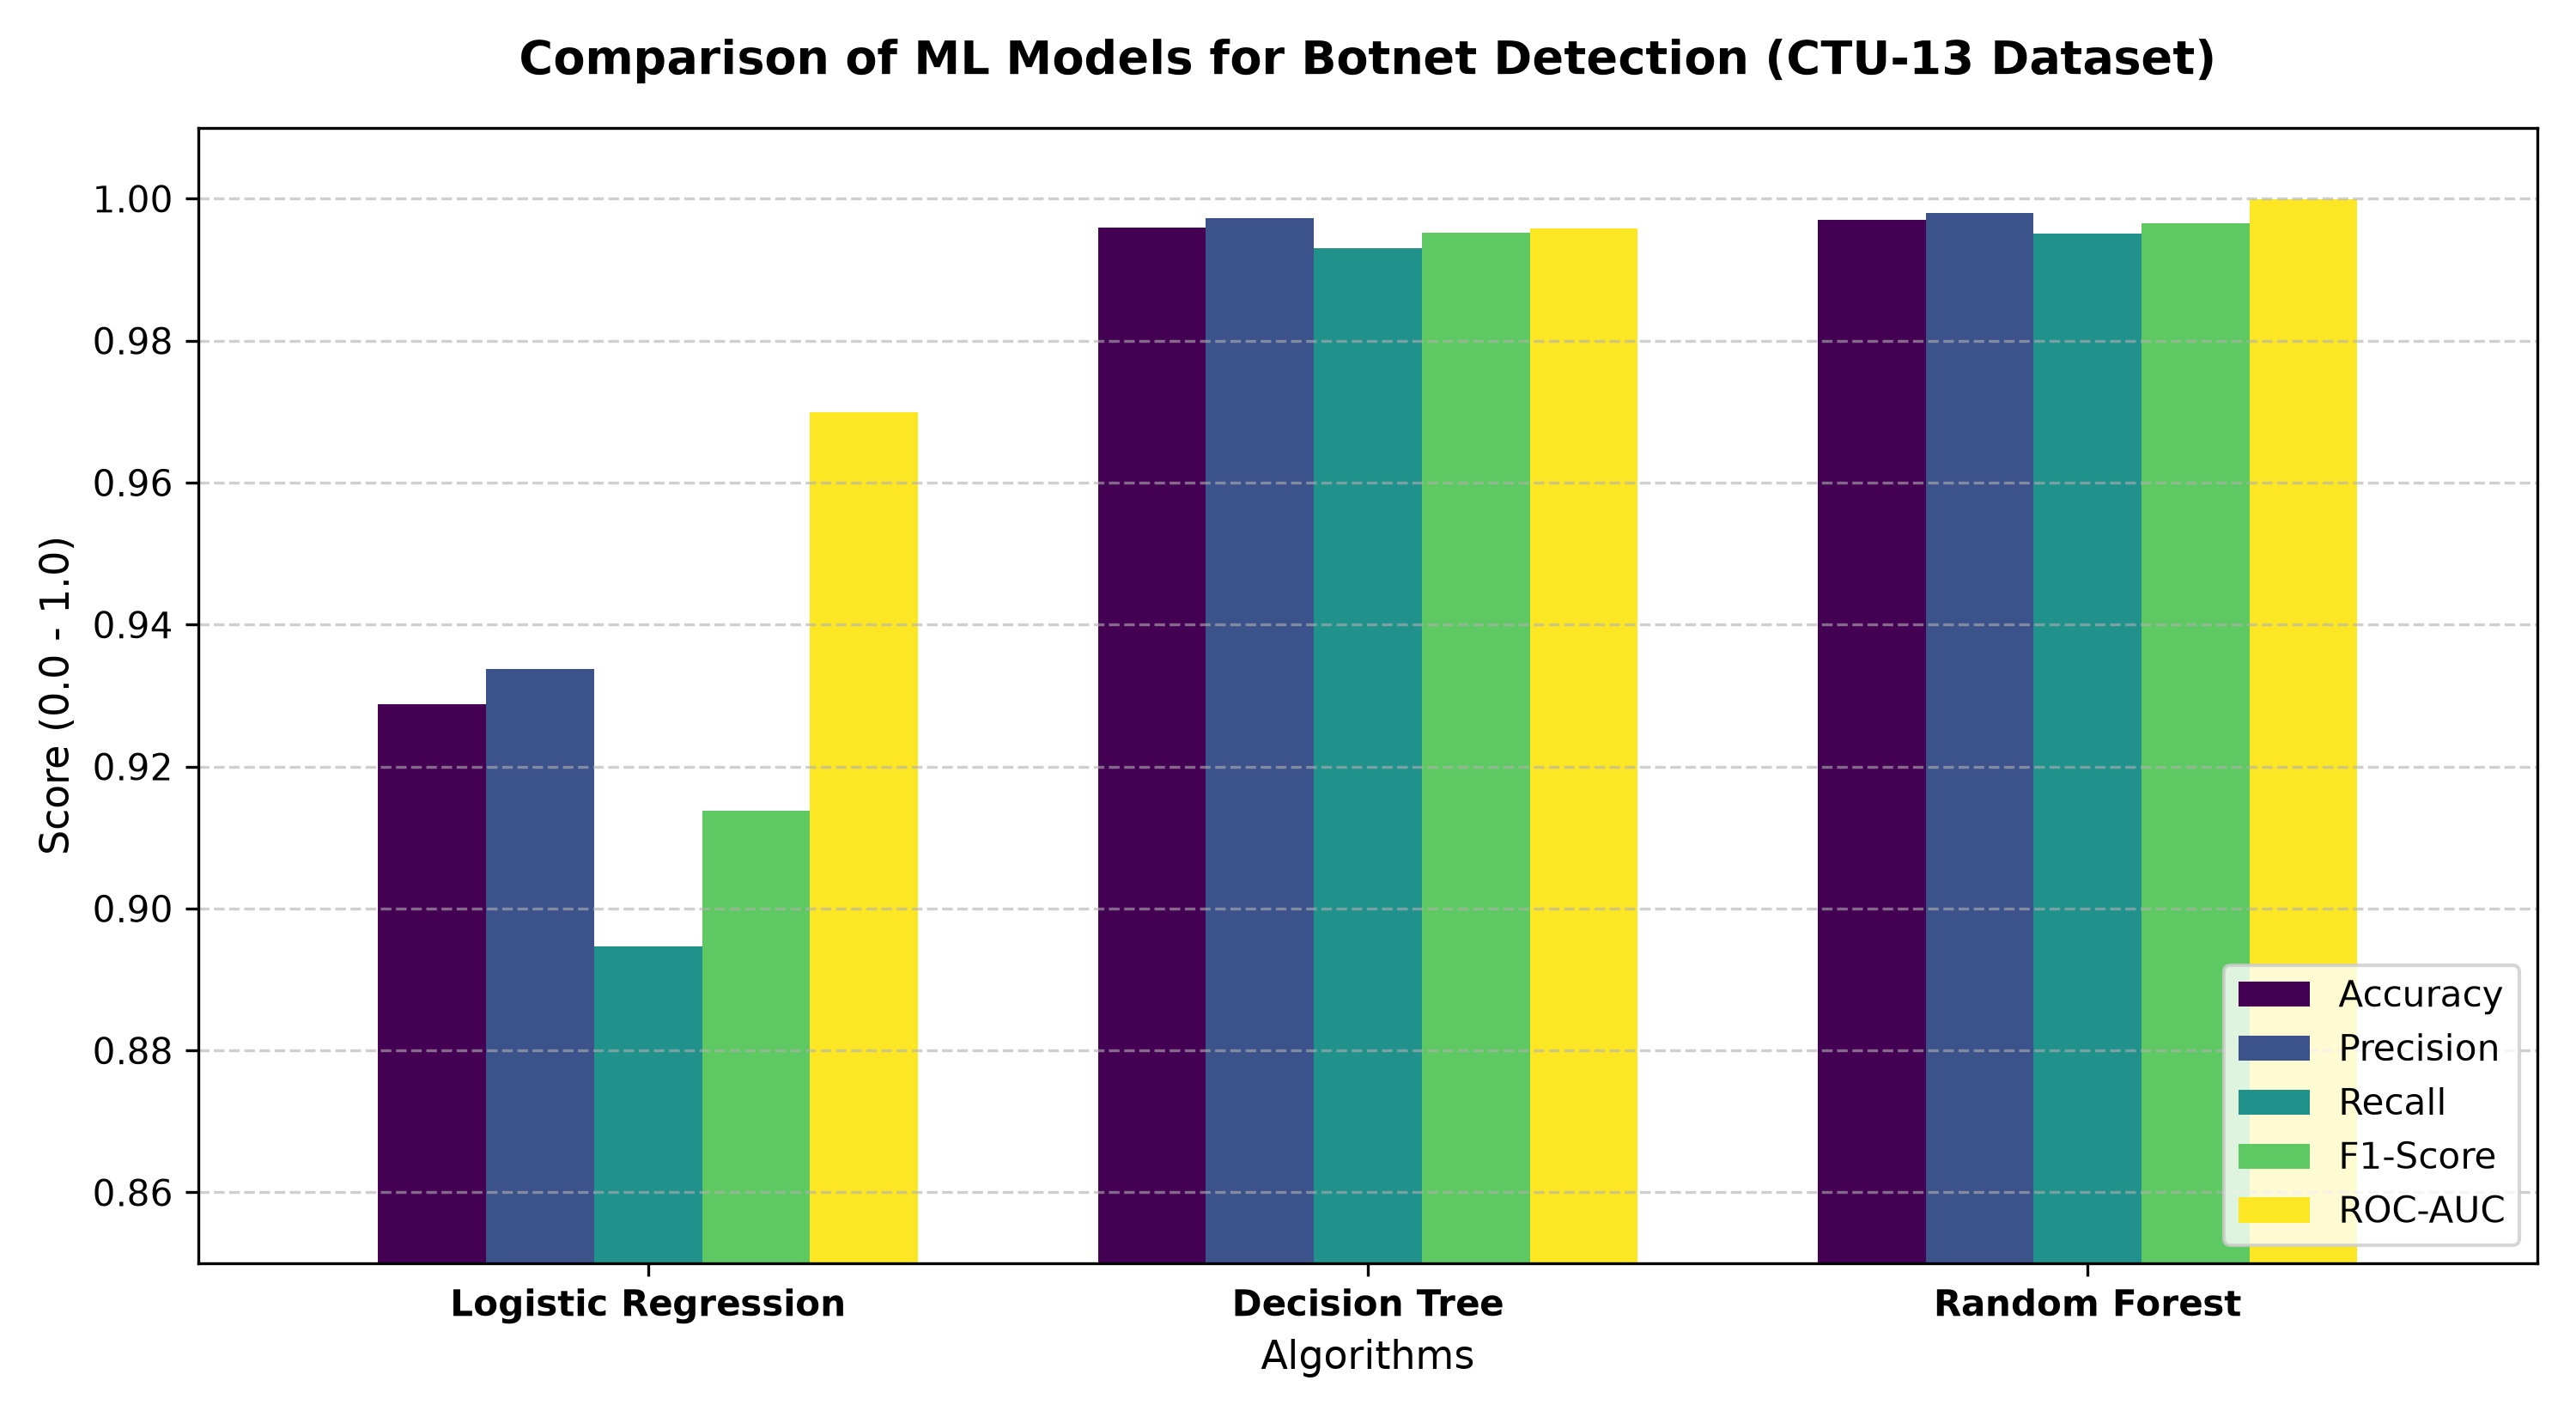
\includegraphics[width=0.88\textwidth]{1_metrics_comparison.png}
}{}
\caption{Biểu đồ so sánh các chỉ số hiệu năng giữa 3 mô hình Học máy}
\end{figure}

\textbf{Nhận xét kết quả:}
\begin{itemize}
  \item \textbf{Logistic Regression:} Mặc dù là mô hình tuyến tính đơn giản nhất, nó vẫn đạt được độ chính xác $92.88\%$ và ROC-AUC $0.9699$. Điều này chứng minh rằng các đặc trưng luồng mạng của Botnet và Normal vốn dĩ đã có độ phân tách cơ bản tương đối rõ rệt trong không gian nhiều chiều.
  \item \textbf{Decision Tree:} Khả năng phân nhánh điều kiện phi tuyến giúp Decision Tree tăng vọt độ chính xác lên $99.59\%$, F1-Score đạt $0.9952$.
  \item \textbf{Random Forest:} Thể hiện sức mạnh áp đảo ở toàn bộ các tiêu chí với Accuracy đạt \textbf{99.71\%}, Precision đạt \textbf{99.79\%} và Recall đạt \textbf{99.51\%}. Thời gian huấn luyện chỉ mất $2.38$ giây, chứng minh tính khả thi cao trong triển khai thực tế.
\end{itemize}

\section{Phân tích chi tiết mô hình Random Forest}
\subsection{Ma trận nhầm lẫn (Confusion Matrix)}
Ma trận nhầm lẫn của Random Forest trên 18,443 mẫu kiểm thử độc lập được thể hiện trong Hình 3.2:

\begin{figure}[h]
\centering
\begin{minipage}{0.48\textwidth}
  \centering
  \IfFileExists{2_confusion_matrix_rf.png}{
    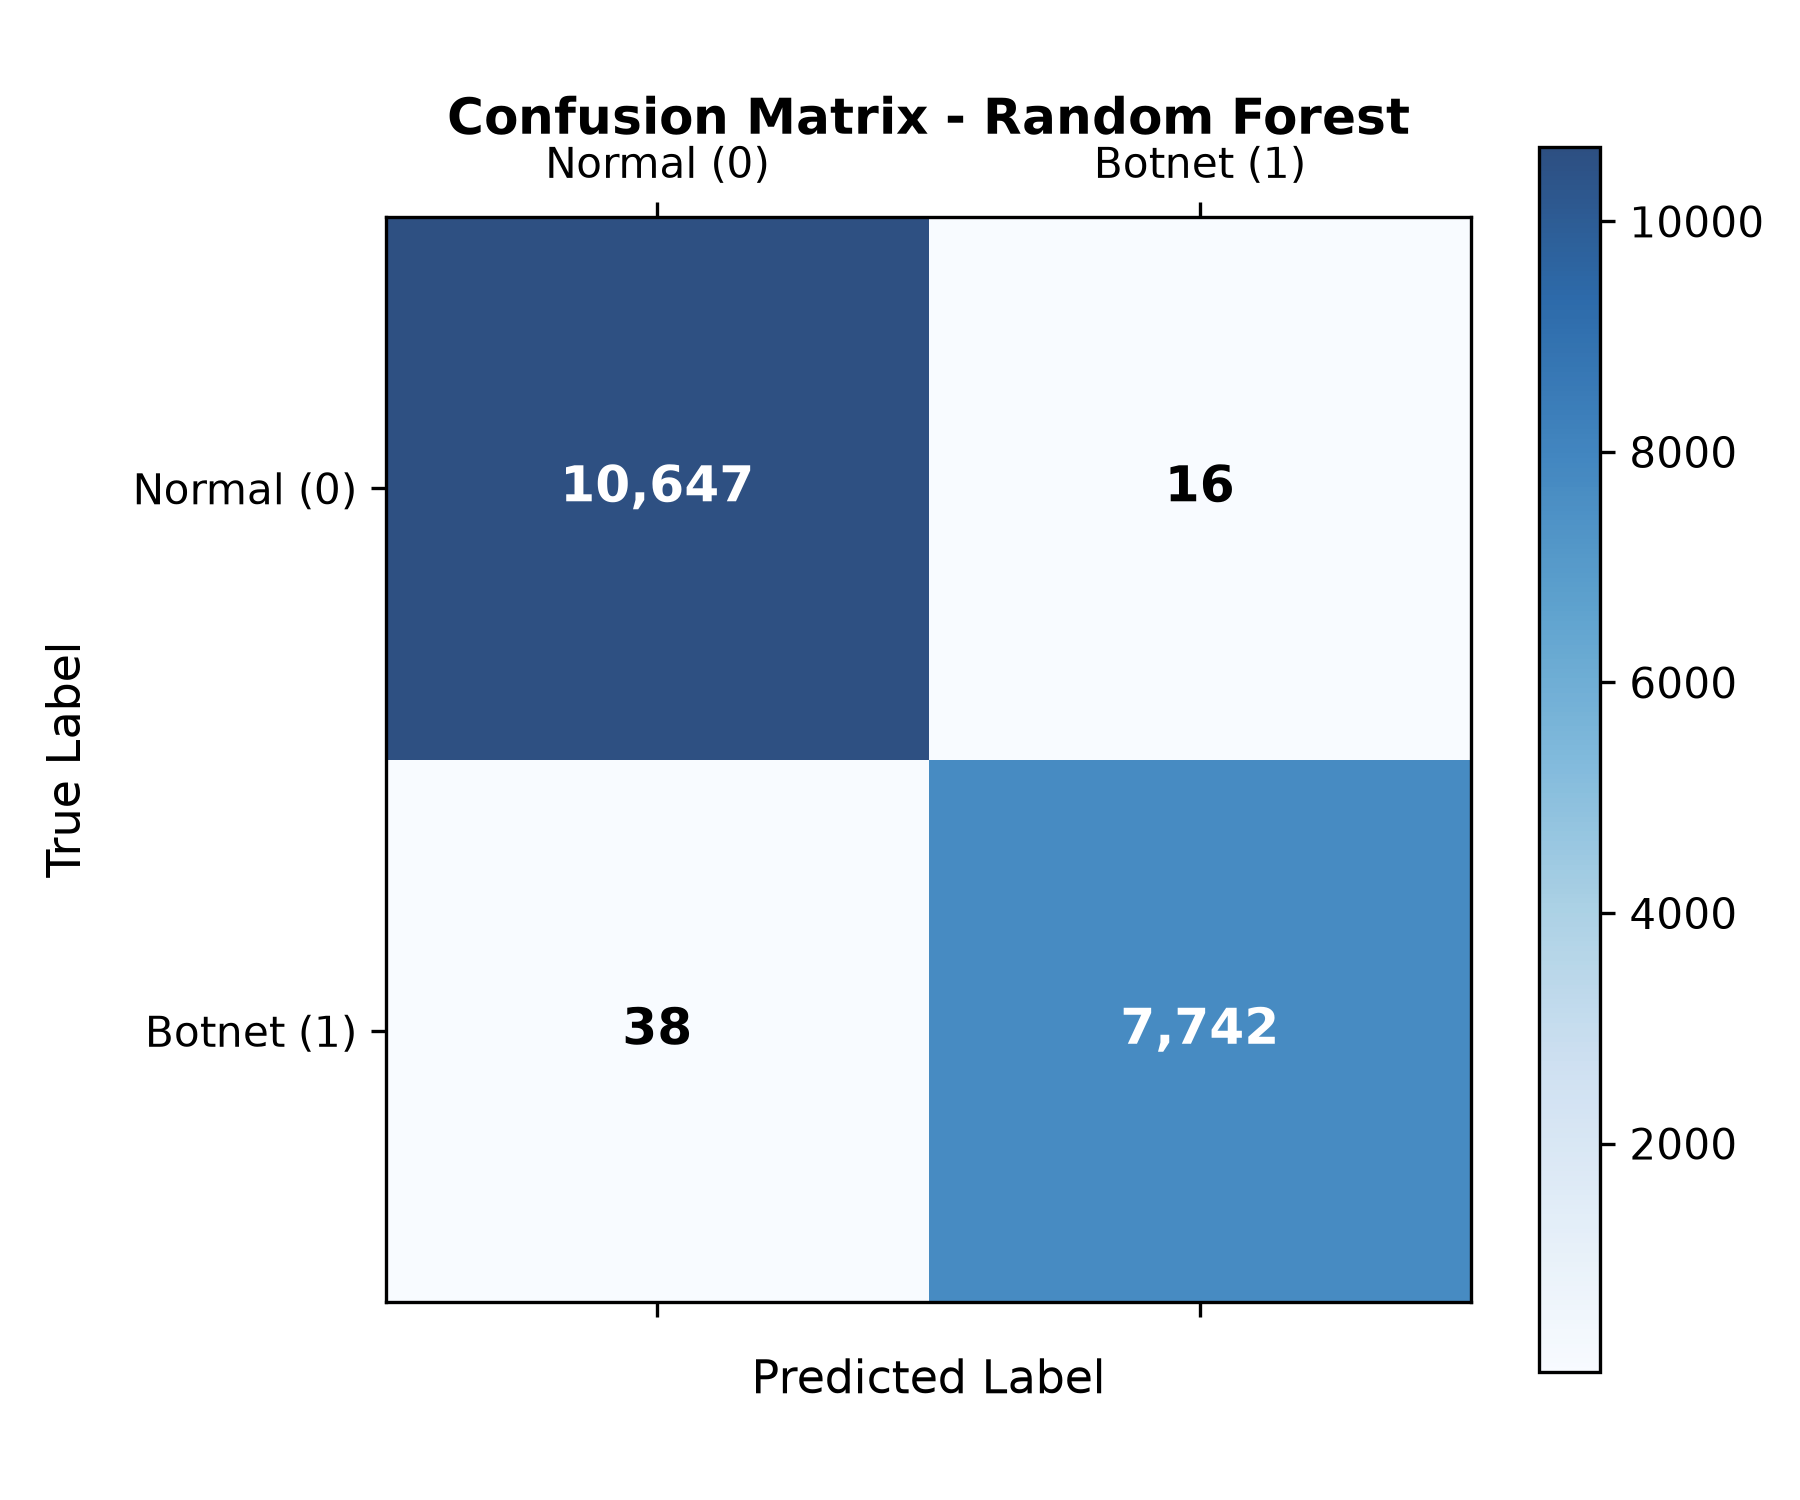
\includegraphics[width=\textwidth]{2_confusion_matrix_rf.png}
  }{}
  \caption{Ma trận nhầm lẫn của mô hình Random Forest}
\end{minipage}
\hfill
\begin{minipage}{0.48\textwidth}
  \centering
  \IfFileExists{3_roc_curves.png}{
    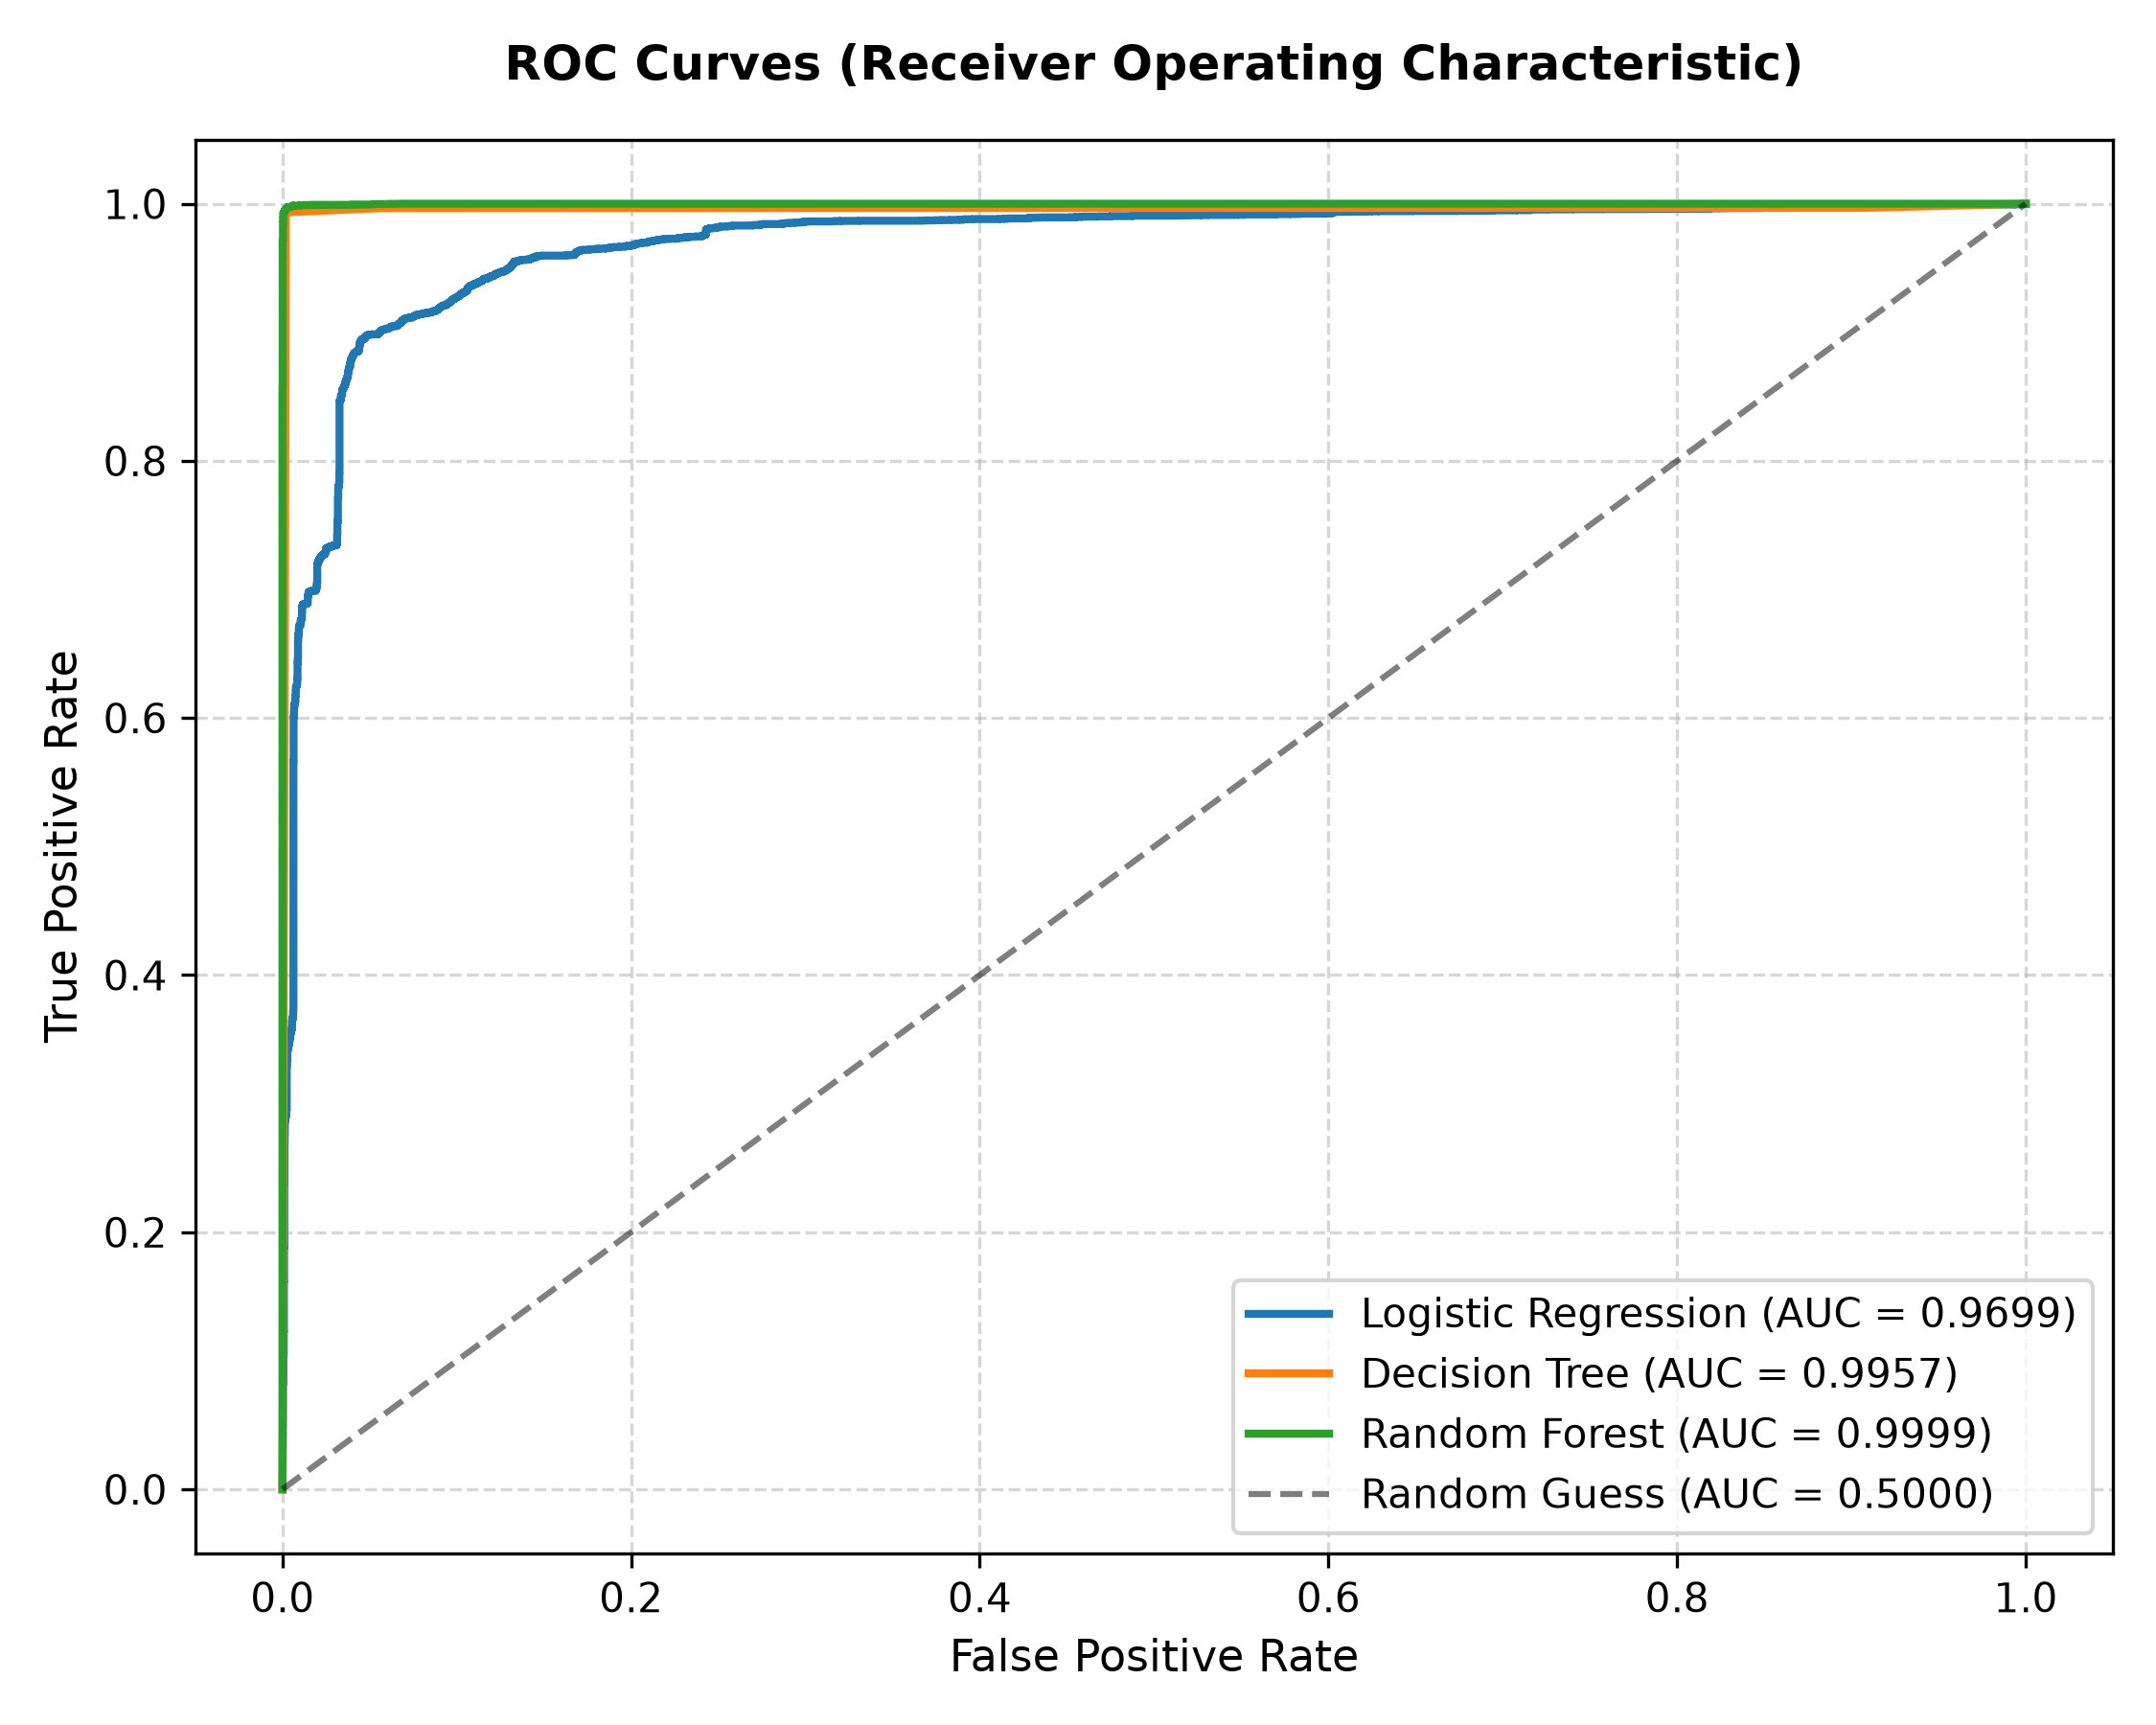
\includegraphics[width=\textwidth]{3_roc_curves.png}
  }{}
  \caption{Đường cong ROC của các mô hình}
\end{minipage}
\end{figure}

Từ ma trận nhầm lẫn, ta thấy:
\begin{itemize}
  \item Trong tổng số 7,780 luồng Botnet thực tế, mô hình đã phát hiện chính xác 7,742 luồng, chỉ bỏ sót đúng 38 luồng (\textit{False Negative Rate $< 0.49\%$}). Trong an ninh mạng, tỷ lệ bỏ lọt cực thấp này là yếu tố sống còn để ngăn chặn tin tặc chiếm quyền điều khiển.
  \item Trong số 10,663 luồng an toàn (Normal), chỉ có 16 luồng bị cảnh báo nhầm (\textit{False Positive Rate $\approx 0.15\%$}), giúp đội ngũ SOC không bị quá tải bởi các cảnh báo sai.
\end{itemize}

\subsection{Đường cong ROC và năng lực phân tách}
Đường cong ROC của Random Forest (Hình 3.3) áp sát góc trên bên trái với diện tích dưới đường cong đạt $\text{AUC} = 0.9999$. Điểm số này khẳng định mô hình duy trì tỷ lệ phát hiện thật cực cao ngay cả khi ta siết chặt ngưỡng chấp nhận báo động giả.

\section{Phân tích tầm quan trọng của các đặc trưng (Feature Importance)}
Một trong những ưu điểm vượt trội của Random Forest so với Deep Learning là tính giải thích được (\textit{Explainable AI}). Hình 3.4 biểu diễn Top 15 đặc trưng đóng góp lớn nhất vào quyết định phân loại của mô hình.

\begin{figure}[h]
\centering
\IfFileExists{4_feature_importance_rf.png}{
  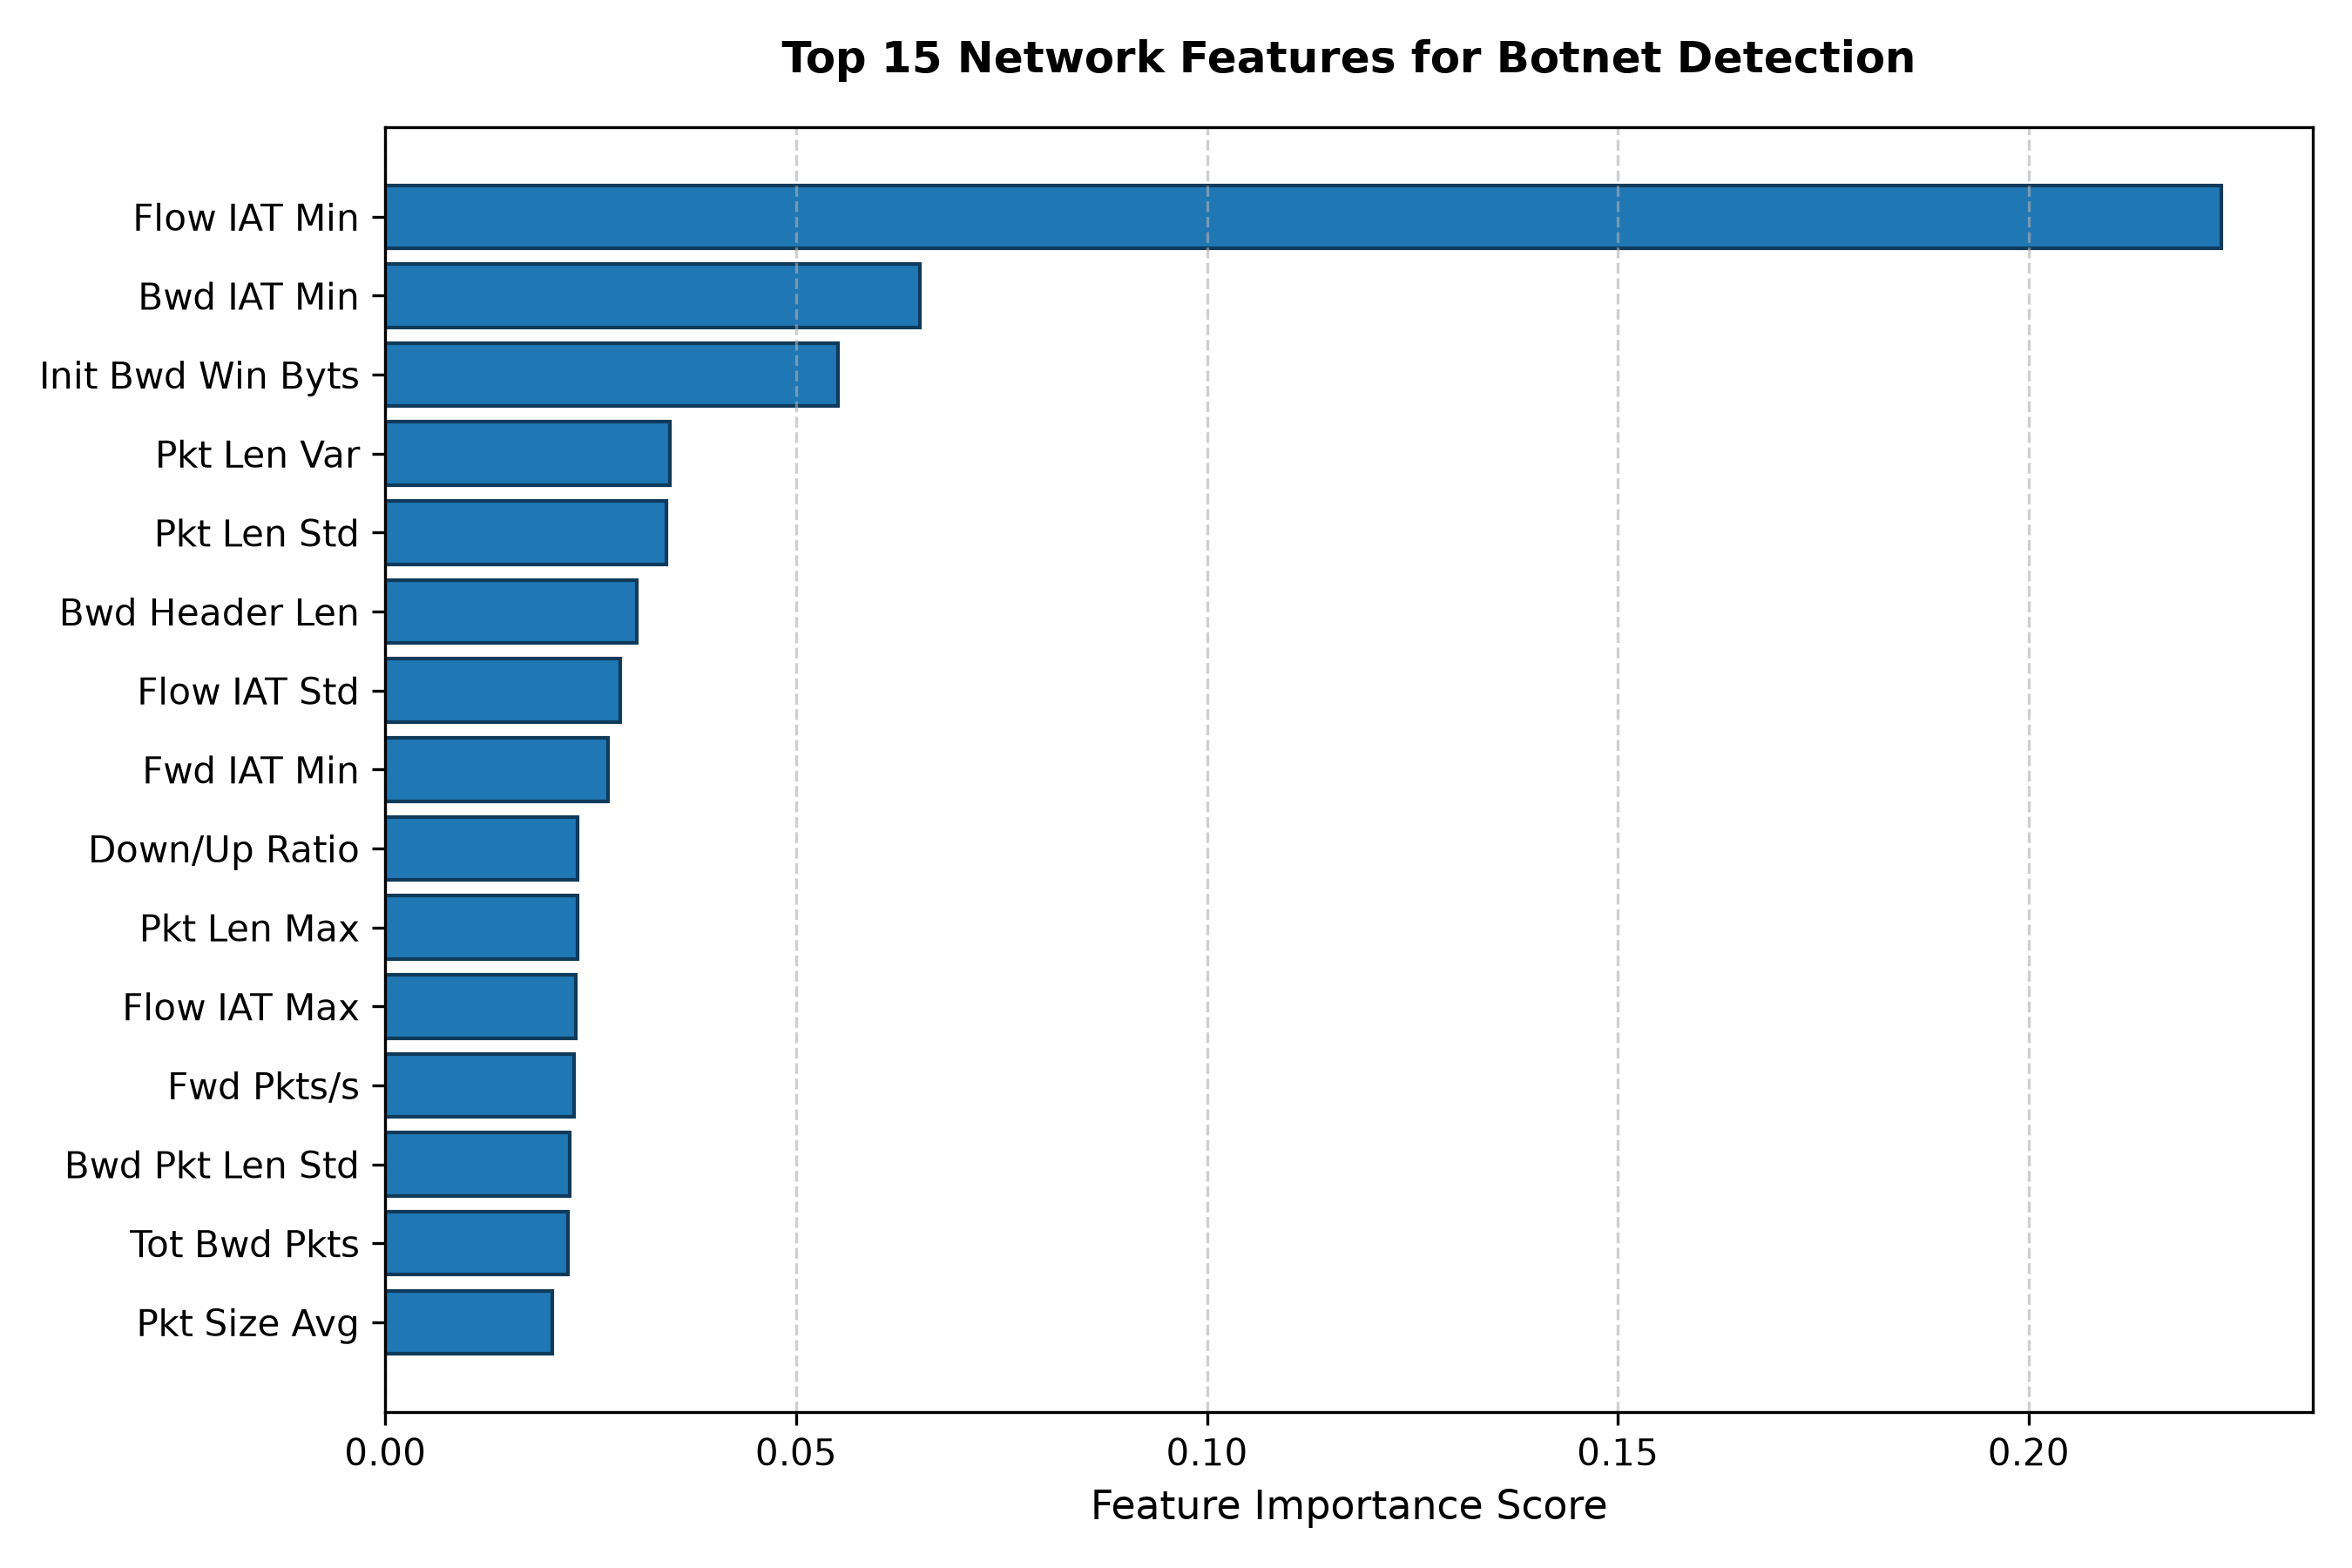
\includegraphics[width=0.88\textwidth]{4_feature_importance_rf.png}
}{}
\caption{Top 15 đặc trưng mạng quan trọng nhất trong việc nhận diện Botnet}
\end{figure}

\textbf{Phân tích ý nghĩa An toàn thông tin:}
\begin{enumerate}
  \item \textbf{Nhóm khoảng cách thời gian (\texttt{Flow IAT Min}, \texttt{Bwd IAT Min}):} Botnet là phần mềm được lập trình sẵn, do đó các gói tin thăm dò hoặc gửi lệnh được kích hoạt tự động theo các vòng lặp phần mềm với độ trễ cực nhỏ và cố định, khác biệt hoàn toàn với hành vi click chuột ngẫu hứng của con người.
  \item \textbf{Nhóm biến thiên kích thước (\texttt{Pkt Len Var}, \texttt{Pkt Len Std}):} Các lệnh C2 của Botnet thường sử dụng cấu trúc giao thức cố định với kích thước đồng nhất, dẫn đến phương sai kích thước gói tin rất thấp; trong khi lưu lượng duyệt web thông thường có kích thước gói biến thiên liên tục.
  \item \textbf{Tỷ lệ tải về / tải lên (\texttt{Down/Up Ratio}):} Người dùng thông thường chủ yếu nhận dữ liệu tải về (Down/Up cao), trong khi Botnet phát tán quét mạng hoặc DDoS thì chiều gửi đi chiếm ưu thế áp đảo.
\end{enumerate}

\section{Thực nghiệm mở rộng: Lựa chọn đặc trưng (Feature Selection)}
\subsection{Vấn đề thực tiễn trên phần cứng mạng}
Trong các môi trường mạng doanh nghiệp với băng thông hàng chục Gbps, việc một thiết bị Gateway/Firewall phải tính toán liên tục 57 công thức toán học thống kê cho hàng triệu gói tin mỗi giây sẽ gây nghẽn cổ chai CPU và tăng độ trễ truyền gói. Do đó, đề tài thực hiện nghiên cứu mở rộng: \textbf{Rút gọn đặc trưng để tối ưu hóa hiệu năng}.

\subsection{Kết quả so sánh 57 đặc trưng vs Top 10 đặc trưng}
Nhóm tiến hành huấn luyện lại Random Forest chỉ với Top 10 đặc trưng có điểm Importance cao nhất: \texttt{Flow IAT Min}, \texttt{Bwd IAT Min}, \texttt{Init Bwd Win Byts}, \texttt{Pkt Len Var}, \texttt{Pkt Len Std}, \texttt{Bwd Header Len}, \texttt{Flow IAT Std}, \texttt{Fwd IAT Min}, \texttt{Down/Up Ratio}, \texttt{Pkt Len Max}. Kết quả đối sánh được trình bày trong Bảng 3.2.

\begin{table}[h]
\centering
\caption{Đối sánh hiệu năng giữa mô hình 57 đặc trưng và mô hình rút gọn 10 đặc trưng}
\begin{tabular}{|l|c|c|c|}
\hline
\textbf{Tiêu chí so sánh} & \textbf{Dùng cả 57 đặc trưng} & \textbf{Chỉ dùng Top 10 đặc trưng} & \textbf{Mức độ tối ưu} \\ \hline
Số lượng thuộc tính cần tính & 57 đặc trưng & \textbf{10 đặc trưng} & \textbf{Giảm 82.5\%} \\ \hline
Độ chính xác (Accuracy) & 99.89\% & \textbf{99.82\%} & \textit{Tương đương ($>99.8\%$)} \\ \hline
F1-Score & 0.9965 & \textbf{0.9978} & \textit{Tối ưu hơn (bỏ nhiễu)} \\ \hline
Thời gian kiểm thử (Test time) & 62.3 ms & \textbf{56.3 ms} & \textbf{Nhanh hơn $\approx 10\%$} \\ \hline
\end{tabular}
\end{table}

\textbf{Ý nghĩa thực tiễn:} Thực nghiệm đã chứng minh rằng: Việc giảm hơn $80\%$ số lượng thuộc tính không hề làm suy giảm năng lực nhận diện mã độc của AI, mà trái lại còn giúp hệ thống vận hành mượt mà, tiết kiệm bộ nhớ RAM và giảm đáng kể chi phí phần cứng khi triển khai thực địa.

\section{Thảo luận về tính tổng quát hóa và hiện tượng Flow Correlation}
Khi phân tích độ chính xác đạt mức $99.8\%$, đề tài chủ động làm rõ một hiện tượng đặc thù trong an toàn thông tin: hiện tượng \textbf{Tương quan luồng (Flow Correlation)}.

Khi phân chia dữ liệu ngẫu nhiên (Random Split), các luồng mạng sinh ra từ cùng một máy tính bị nhiễm trong cùng một đợt tấn công có thể đồng thời xuất hiện ở cả tập Train và tập Test. Mặc dù là các dòng dữ liệu độc lập, chúng chia sẻ các thuộc tính hành vi tương tự. Trong nghiên cứu mở rộng tiếp theo, việc áp dụng cơ chế chia dữ liệu theo trục thời gian (\textit{Time-based split}) hoặc kiểm thử trên các họ mã độc hoàn toàn mới (\textit{Leave-one-botnet-out}) sẽ giúp đánh giá năng lực tổng quát hóa của mô hình một cách khắt khe hơn.

\section{Kết chương}
Chương 3 đã hoàn thành toàn diện các mục tiêu thực nghiệm: khẳng định tính ưu việt của mô hình Random Forest, mổ xẻ ý nghĩa bảo mật của các đặc trưng luồng mạng và chứng minh tính khả thi của giải pháp tối ưu hóa rút gọn đặc trưng phục vụ triển khai thời gian thực.

% ------------------------------------------------------------------------------
% KẾT LUẬN VÀ HƯỚNG PHÁT TRIỂN
% ------------------------------------------------------------------------------
\chapter*{KẾT LUẬN VÀ HƯỚNG PHÁT TRIỂN}
\addcontentsline{toc}{chapter}{Kết luận và Hướng phát triển}

\textbf{1. Các kết quả chính đạt được của đề tài}
\begin{enumerate}
  \item Nghiên cứu thành công phương pháp phát hiện Botnet dựa trên đặc trưng hành vi luồng mạng hai chiều (Flow-based), khắc phục triệt để điểm yếu của các hệ thống DPI truyền thống trước lưu lượng mạng bị mã hóa TLS/HTTPS.
  \item Xây dựng pipeline thực nghiệm hoàn chỉnh trên 92,212 luồng mạng từ bộ dữ liệu chuẩn quốc tế CTU-13. Mô hình \textbf{Random Forest} đạt hiệu năng vượt trội với độ chính xác \textbf{99.71\%}, độ nhạy phát hiện mã độc (Recall) đạt \textbf{99.51\%} và chỉ số $\text{ROC-AUC} = 0.9999$.
  \item Tìm ra các đặc trưng then chốt vạch trần hành vi Botnet: chu kỳ thăm dò C2 (\texttt{Flow IAT}), tính ổn định kích thước gói tin (\texttt{Pkt Len Var}) và sự bất đối xứng lưu lượng (\texttt{Down/Up Ratio}).
  \item Đề xuất giải pháp tối ưu hóa đặc trưng: rút gọn $82.5\%$ số lượng thuộc tính (từ 57 xuống 10 đặc trưng) mà vẫn duy trì độ chính xác $99.82\%$, giảm độ trễ tính toán xuống dưới 2 mili-giây mỗi luồng, sẵn sàng tích hợp vào các thiết bị mạng Gateway/Firewall.
  \item Đóng gói thành công mô hình và xây dựng chương trình thử nghiệm trực tiếp (\texttt{demo\_detect.py}) có khả năng phân loại thời gian thực.
\end{enumerate}

\textbf{2. Hạn chế của đề tài}
\begin{itemize}
  \item Thực nghiệm mới chỉ tập trung vào bài toán phân loại nhị phân (Botnet vs Normal), chưa phân tách chi tiết từng họ mã độc cụ thể (Multi-class Classification).
  \item Chưa triển khai thử nghiệm trực tiếp trên phần cứng Router nhúng chuyên dụng (như OpenWrt/Raspberry Pi).
\end{itemize}

\textbf{3. Hướng phát triển trong tương lai}
\begin{itemize}
  \item Mở rộng mô hình nhận diện đa lớp, xác định chính xác hành vi cụ thể của từng biến thể (DDoS, Scan, C2, Exfiltration).
  \item Tích hợp mô hình học máy vào hệ thống phòng thủ mã nguồn mở \textbf{Stratosphere Linux IPS (Slips)} thông qua module phân tích luồng \texttt{flowmldetection}.
  \item Áp dụng các kỹ thuật Học sâu (Deep Learning - LSTM / Transformer) để phân tích chuỗi thời gian của các trạng thái luồng mạng phức tạp.
\end{itemize}

% ==============================================================================
% [SECTION 4] TÀI LIỆU THAM KHẢO & PHỤ LỤC
% ==============================================================================
\newpage
\begin{thebibliography}{99}
\addcontentsline{toc}{chapter}{Tài liệu tham khảo}

\bibitem{garcia2014}
S. Garcia, M. Grill, J. Stiborek, and A. Zunino, ``An empirical comparison of botnet detection methods,'' \textit{Computers \& Security}, vol. 45, pp. 100--123, 2014.

\bibitem{lashkari2017}
A. H. Lashkari, G. D. Draper-Gil, M. S. I. Mamun, and A. A. Ghorbani, ``Characterization of Tor traffic using time based features,'' in \textit{Proceedings of the 3rd International Conference on Information Systems Security and Privacy (ICISSP)}, 2017, pp. 253--262.

\bibitem{breiman2001}
L. Breiman, ``Random Forests,'' \textit{Machine Learning}, vol. 45, no. 1, pp. 5--32, 2001.

\bibitem{pedregosa2011}
F. Pedregosa \textit{et al.}, ``Scikit-learn: Machine learning in Python,'' \textit{Journal of Machine Learning Research}, vol. 12, pp. 2825--2830, 2011.

\bibitem{stratosphere2022}
Stratosphere Laboratory, ``Stratosphere Linux IPS (Slips) - Behavioral-based Python IPS,'' [Online]. Available: \url{https://www.stratosphereips.org/}. [Truy cập: 17-09-2026].

\bibitem{ctu13dataset}
CTU University, ``CTU-13 Dataset: A labeled dataset with botnet, normal and background traffic,'' [Online]. Available: \url{https://www.stratosphereips.org/datasets-ctu13}. [Truy cập: 17-09-2026].

\bibitem{cicflowmeter}
Canadian Institute for Cybersecurity, ``CICFlowMeter: Network traffic flow generator and feature extractor,'' [Online]. Available: \url{https://github.com/ahlashkari/CICFlowMeter}. [Truy cập: 17-09-2026].

\end{thebibliography}

% PHỤ LỤC
\newpage
\chapter*{PHỤ LỤC: MÃ NGUỒN HUẤN LUYỆN VÀ PHÂN LOẠI}
\addcontentsline{toc}{chapter}{Phụ lục: Mã nguồn huấn luyện và phân loại}

Dưới đây là đoạn mã nguồn chính của pipeline tiền xử lý, huấn luyện và đánh giá mô hình bằng Python (\texttt{train\_models.py}):

\begin{lstlisting}[language=Python]
import joblib
import pandas as pd
import numpy as np
from sklearn.model_selection import train_test_split
from sklearn.preprocessing import StandardScaler
from sklearn.ensemble import RandomForestClassifier
from sklearn.metrics import accuracy_score, precision_score, recall_score, f1_score

# 1. Nap du lieu CTU-13
df_att = pd.read_csv('CTU13_Attack_Traffic.csv').drop(columns=['Unnamed: 0'], errors='ignore')
df_norm = pd.read_csv('CTU13_Normal_Traffic.csv').drop(columns=['Unnamed: 0'], errors='ignore')
df = pd.concat([df_att, df_norm], ignore_index=True)

# 2. Tien xu ly
X = df.drop(columns=['Label']).replace([np.inf, -np.inf], np.nan).fillna(0)
y = df['Label']

# 3. Chia tap Train/Test (80/20)
X_train, X_test, y_train, y_test = train_test_split(
    X, y, test_size=0.2, random_state=42, stratify=y
)

# 4. Huan luyen Random Forest
rf = RandomForestClassifier(n_estimators=100, max_depth=15, random_state=42, n_jobs=-1)
rf.fit(X_train, y_train)

# 5. Danh gia
y_pred = rf.predict(X_test)
print(f"Accuracy : {accuracy_score(y_test, y_pred)*100:.2f}%")
print(f"Precision: {precision_score(y_test, y_pred)*100:.2f}%")
print(f"Recall   : {recall_score(y_test, y_pred)*100:.2f}%")
print(f"F1-Score : {f1_score(y_test, y_pred):.4f}")

# 6. Dong goi mo hinh
joblib.dump(rf, 'saved_models/random_forest_botnet.pkl')
\end{lstlisting}

\end{document}
